\chapter{Methodology Part 1: Geometry Representation and Point Placement}

In this section, we will talk about the initial import of surface triangulation and storing the surface as a collection of bezier surface patches. Then, the point placement subroutine is explained which decides the mesh element structure. Lastly, a small discussion on the local mesh element quality improvement is added to explain the face swapping algorithm. 

\section{Surface Import}

\subsection{Surface Representation - A brief overview}

Surfaces can be represented in various forms. A surfaces can be represented with their implicit form, given by
\begin{equation}
F(x, y, z) = 0
\label{implicitSurface}
\end{equation}
where, the surface is defined as the locus of points whose coordinates $(x, y, z)$ satisfly the above equation. If the equation \ref{implicitSurface} is linear in variables $x, y, and z$, it represents a plane. If the equation \ref{implicitSurface} is of second degree in $x, y, \textnormal{ or } z$, it represents quadrics. If the implicit equaiton can be solved for one of the variables as a function of of the other two, say $z$ is solved in terms of $x$ and $y$, we obtain an explicit surface
\begin{equation}
z = F(x,y)
\end{equation}

Figure \ref{fig-imex} shows an implicit and an explicit surface together with their mathematical formulations.

\begin{figure}
  \begin{subfigure}{0.5\linewidth}
  \centering
  \includegraphics[width=0.9\linewidth]{img/m1/explicit.png}
  \caption{}
  \label{fig-explicit}
  \end{subfigure}
  \begin{subfigure}{0.5\linewidth}
    \centering
    \includegraphics[width=0.8\linewidth]{img/m1/implicit.png}
    \caption{}
  \end{subfigure}
  \caption{(a) An explicit surface, given by $z = \cos ((x+y))+\frac{x^{2}}{6}-\frac{y^{2}}{6}$. (b) An implicit surface, given by $2 y\left(y^{2}-3 x^{2}\right)\left(1-z^{2}\right)+\left(x^{2}+y^{2}\right)^{2}-\left(9 z^{2}-1\right)\left(1-z^{2}\right)=0$. }
  \label{fig-imex}
\end{figure}

Apart from the explicit and implicit forms, surfaces can also be represented in their parametric form. The coordinates of a point $(x,y,z)$ of the surface patch are expressed as functions of parameters $u$ and $v$ in a closed rectangle:

\begin{equation}
x=x(u, v), \quad y=y(u, v), \quad z=z(u, v), \quad u_{1} \leq u \leq u_{2}, \quad v_{1} \leq v \leq v_{2}.
\end{equation}

In vector notation, the parametric surface can be specified by a vector-valued function

\begin{equation}
\mathbf{r}=\mathbf{r}(u, v)
\end{equation}

The parametric representation of surfaces is the most versatile out of the three. It is axis independent and is highly flexible in terms of defining complex intersections and point classification. It is generally easier to manipulate free-form shapes in parametric form than implicit or explicit forms  \cite{patrikalakis2009shape}. Hence, most CAD packages use the parametric form of surfaces. A bezier surface patch and NURBS are examples of the parametric form of a surface.

\subsection{Surface File Format}
\label{surfaceFileFormat}

\begin{figure}
  \centering
  \includegraphics[width=\linewidth]{img/m1/tessellation.png}
  \caption{The perfect spherical surface on the left is approximated by tessellations. The figure on the right uses big triangles, resulting in a coarse model. The figure on the center uses smaller triangles and achieves a smoother approximation \cite{fileFormat}}
  \label{fig-tesellation}
\end{figure}

Given a free-form 3D surface geometry, various CAD packages could be used to encode it and store it in a file. Encoding the geometry using an approximate mesh is one of the most common methods adopted to store a surface geometry. An approximate mesh is created by covering the surface geometry with a series of tiny imaginary polygons. Triangles are the most common polygon used for mesh generation. The encoded surface mesh can be stored in a file for sharing and future reference purposes. These files store the vertices of the triangles as well as the outward normal directions to the triangles. This process of tiling a surface with non-overlapping geometric shapes is also known as tessellation. Hence, the file formats used for storing the surface representation are called tessellated formats.

Due to the independent development of various CAD packages, a plethora of surface file formats are present in the mesh generation ecosystem. Many of these formats, such as DWG file format by AutoCAD and BLEND file format by Blender\cite{blender} are proprietary. Hence, many of these cannot be shared between people working on different CAD packages. Neutral file formats are used to solve this problem. These formats can be shared easily among people working on different meshing software. One of the most common neutral surface file formats is the STL (STereoLithography) file format. This format is compatible with most of the CAD and visualization softwares. Hence, we use the STL file format to import the surface geometry into our mesh generation algorithm.

An STL file stores the surface as a triangulated mesh. The following information is stored for all the triangles in the STL file format:

\begin{enumerate}
  \item The coordinates of the vertices
  \item The components of the unit normal vector to the triangle pointing outwards with respect to the 3D model
\end{enumerate}

Innumerable software packages are available online which can be used to triangulate a surface (see \cite{meshSoftware} for a list of such software). A fine triangular mesh can be considered as an approximate encoding of a given surface geometry. The approximation could be improved by increasing the number of triangles or decreasing their size. However, using smaller triangles results in larger number of triangles needed to tile the surface. This increases the mesh file size. Hence, a user should define the mesh element size according to the kind of refinement needed.

\section{Surface Import and Segmentation using the Common Geometry Module (CGM)}

As explained in Section \ref{surfaceFileFormat}, we import the surface geometry as a triangulation from an STL file. The Common Geometry Module (CGM) package is used to read the surface file and store the triangulation for further processing. The triangulated surface is stored as a collection of segmented sub-surfaces. The segmentation in CGM is done by identifying features in the surface. The only input parameter for surface segmentation accepted by CGM is the feature angle. We keep this feature angle value to be 135{$^\circ{}$}. This value helps us to identify sharp corners and edges on the surface. Figure \ref{fig-surfSegment} shows a surface triangulation of an arbitrary mechanical part. The surface triangulation is segmented into 10 sub-surfaces, which are identified by the sharp features on the surface. Four of these are shown in outline in the figure.

Each triangle imported in CGM is stored as a quartic-Bezier patch. We will refer to the imported triangulation as $T$ and the underlying Bezier surface representation as $S$. The underlying Bezier surface representation $S$ is considered to be the ground truth for the surface mesh and the mesh points are placed directly over $S$. The initial imported triangulation $T$ is taken as the initial mesh. 

Using $T$ as our initial mesh means that we can use a closed advancing layer mesh generation methodology. There are advantages and disadvantages of using such a methodology. Open advancing layer method requires less work overall to generate the mesh as there are no points to delete or reconnect to, ahead of the front. On the other hand, handling mesh layer collisions is  more tricky in open advancing layer method as no connectivity information is available ahead of the front in such methods. This leads to abrupt layer closures, which are undesirable in an anisotropic mesh.

Closed advancing layer mesh generation method generates a valid surface mesh at any given point in time during the mesh generation process. Hence, there is more flexibility in terms of when to stop the marching layers and output the mesh in its current state. Additionally, connectivity information is known ahead of the front. This information is helpful while tackling front collisions. This will be explained in more detail when we talk about handling front collisions in *ref*.

\begin{figure}
\centering
\begin{subfigure}{.5\textwidth}
  \centering
  \includegraphics[width=.8\linewidth]{img/m1/surfSegmentation/surf0.eps}
  \caption{}
  \label{surf0}
\end{subfigure}%
\begin{subfigure}{.5\textwidth}
  \centering
  \includegraphics[width=.8\linewidth]{img/m1/surfSegmentation/surf3.eps}
  \caption{}
  \label{surf1}
\end{subfigure}
\begin{subfigure}{.5\textwidth}
  \centering
  \includegraphics[width=.8\linewidth]{img/m1/surfSegmentation/surf5.eps}
  \caption{}
  \label{surf2}
\end{subfigure}%
\begin{subfigure}{.5\textwidth}
  \centering
  \includegraphics[width=.8\linewidth]{img/m1/surfSegmentation/surf7.eps}
  \caption{}
  \label{surf3}
\end{subfigure}
\caption{An example input triangulation of an arbitrary mechanical part. Four of the segmented surfaces are outlined.}
\label{fig-surfSegment}
\end{figure}

\subsection{Advancing Layer Initialization}

Sharp features of the imported surface are used by CGM to segment the surface. The boundary curves of the segmented surface denote these sharp features. For the purpose of this thesis, we consider these identified boundary curves as the initial front of the mesh. In other words, the boundary curves of the segmented surfaces (or sub-surfaces) serve as the zeroth layer of the advancing layer surface mesh.

Picking the boundary curves of the sub-surfaces to serve as the initial front helps us create anisotropy normal to these boundary curves. This way, desired refinement can be obtained normal to these boundary curves, which is a desirable feature as these boundary curves define the surface features.

The discretization of the boundary curves imported along with the surface triangulation defines the refinement and gradation along the boundary curves (or along the zeroth front). Hence, the refinement and gradation along the boundary curves of the surface is defined by the input triangulation and is up to the user to vary. The surface mesh generated by EDAMSurf hence provides with anisotropy along the normal direction (on the surface) to these boundary curves of the sub-surfaces.

We chose the boundary curves identified by CGM to serve as the zeroth layer of EDAMSurf. However, the initial front could be chosen to be something else without affecting the rest of the mesh generation procedure. For eg. curves along high principal curvature directions on the surface could be added to the zeroth layer of the mesh to get the required anisotropy along highly curved regions of the surface. This is a work in progress and will be added to EDAMSurf in the future.

\section{Point Placement}

After importing the surface triangulation, we have a valid underlying surface representation with us. Also, segmented sub-surfaces and their boundaries curves provide us with the boundaries we need to march off of. Each vertex on these boundary curves is extruded in two directions, one each for the sub-surfaces which share the boundary point. To make things simpler, two copies of each boundary vertex (a vertex on a boundary curve) are created and associated with the two sub-surfaces which share the vertex. This untangles the process of generating the surface mesh of the two sub-surfaces, which can now be meshed independently. Later, when we need to output the final surface mesh, these copies of vertices are recombined.

Meshing sub-surfaces independently has several advantages. If one sub-surface mesh fails to generate, other sub-surfaces would still continue to generate the advancing layer mesh. Different layer on layer \textit{growth ratios} can be used for different sub-surfaces, hence providing the flexibility to choose different anisotropy  for each sub-surface. Also, parallelisation of the surface mesh generation subroutine would be simpler. From here onwards,  the discussion would focus on generating the mesh for a single sub-surface, which is a segment of the complete surface. 

The mesh generation routine starts by initializing the front as the boundary curves of each sub-surface. All the boundary points are marked as candidate marching points and form the starting layer in the mesh. The points at the boundary curves of the sub-surfaces serve as the parent points for the first layer inserted into the mesh.

The data structure created to store a vertex on the advancing front of the mesh also stores the edges adjacent to that vertex so as to identify the marching directions. Hence, the extrusion direction or marching direction of a point is obtained from the location of the vertex, its adjacent edges, and the underlying sub-surface which is being meshed. The extrusion direction calculation procedure is explained in detail in the next subsection.

Similar to the vertices on the boundary curves, edges on the boundary curves are also stored in two copies, one for each sub-surface associated with that edge. Each edge on the advancing layer stores the direction into the interior of the sub-surface it bounds with respect to the surface normal. In other words, the edge datastructure stores its orientation relative to the sub-surface associated with it. As the sub-surfaces sharing a common boundary curve are meshed independently, it is easy to identify the normal to an edge along the sub-surface for advancing the front in the mesh generation algorithm.

%\begin{lstlisting}[language=cpp,caption={Caption}, frame=bt, numbers=none]
%// Class defining a vertex on the advancing layer
%class edamSurfVert {
%public:
%  int index;  
%  
%}
%\end{lstlisting}

\subsection{Extrusion Direction and Length} \label{advancing-layer}

For each of the sub-surfaces of the geometry, the advancing layer routine iteratively picks a point from its boundary and extrudes it in a given direction. After evaluating the extruded point, we project the point onto the underlying surface. This process is set up to be of two steps for simplicity, accuracy and computational efficiency as will be explained later.

\begin{figure}
\centering
\begin{subfigure}{0.5\textwidth}
  \centering
  \includegraphics[trim={2cm 0 2cm 0},clip,width=\linewidth]{img/m1/pointPlacement.png}
  \caption{}
  \label{fig-pointPlacement1}
\end{subfigure}%
\begin{subfigure}{0.5\textwidth}
  \centering
  \includegraphics[width=\linewidth]{img/m1/pointProjection.png}
  \caption{}
  \label{fig-pointPlacement2}
\end{subfigure}
\begin{subfigure}{0.5\textwidth}
	\centering
	\includegraphics[width=\linewidth]{img/m1/pointInsertion.png}
	\caption{}
	\label{fig-pointPlacement3}
\end{subfigure}%
\begin{subfigure}{0.5\textwidth}
	\centering
	\includegraphics[width=\linewidth]{img/m1/localReconnection.png}
	\caption{}
	\label{fig-pointPlacement4}
\end{subfigure}
\caption{(a) Calculation of the extrusion direction of vertex P at the boundary curve of the sub-surface. (b) Projection of the extruded vertex $K$ onto the underlying surface. The projected vertex is marked $Q$. (c) Insertion of the new vertex $Q$ in the triangulation $T$. Red dotted lines denote the new edges created in the mesh. (d) One of the edges next to $Q$ is swapped so as to improve the quality of the mesh.}
\label{fig-point}
\end{figure}

In the first step, we extrude the parent point to get the extruded point. We would interchangeably call the extruded points as the kid points as they represent the successors of their parent points from the previous layer. The direction of this extrusion is set up to be the average of the normals of the parent vertex's adjacent edges in the tangential plane of the sub-surface. In other words, the normals of the adjacent two edges of a vertex on the underlying sub-surface are averaged to get the extrusion direction.

Consider Figure \ref{fig-pointPlacement1}. The initial input triangulation is marked $T$ and the Bezier surface representation is marked $S$. Point $P$ is on the boundary curve of the surface. We need to find the extrusion direction of P to know where its kid will be located. In the underlying triangulation $T$, $PB$ and $PA$ are the edges adjacent to $P$ on the boundary of the surface $S$. We first find the mid-points of quartic-Bezier curves $PB$ and $PA$ which are constructed by CGM as a part of constructing the quartic-Bezier triangular surface patches from the underlying triangulation $T$. Next, we find the normal directions on the surface at these mid-points. The normal directions are carefully queried from the sub-surface which is being meshed currently. The normal directions are labeled as $N_b$ and $N_a$ in the figure. We take the cross product of the vector $PB$ with $N_b$ to get the direction $T_b$. The vector $T_b$ is normal to the edge $PB$ as well as tangential to the surface $S$. Similarly, we find the vector $T_a$, which is normal to the edge $PA$ and tangential to surface $S$. The direction of extrusion $\overrightarrow{PK}$ is chosen to be the average of the direction of $T_a$ and $T_b$.

The \textit{initial extrusion length} is an input parameter provided by the user. This length is used as the extrusion length when the boundary points are extruded for the first time to the interior of the surface. The initial extrusion length can vary with boundary vertices as the points are extruded independently. Hence, this extrusion length can either be supplied by the user for all the points of the boundary separately or as a single value for all the boundary points. To obtain the best quality quadrilateral elements, we scale the extrusion length at a given vertex on the advancing layer with respect to the interior angle between the direction vectors $T_a$ and $T_b$. If the vertex is a concave corner vertex, the extrusion length is increased so as to create good quality quad elements in the next layer. Scaling extrusion length for concave vertices also helps in avoiding immediate front collapse. This process is described in detail in Section \ref{extrusionLengthScaling}.%and vice-versa for convex corner vertices. Also, if the vertex is a convex corner, additional marching directions are added so as to sufficiently refine the interior domain of the surface. The number of additional marching directions added depends on the convexity of the vertex. If we have $n$ marching directions for a point, the angle between the adjacent edges would be divided into $n+1$ angles to get the marching directions for the $n$ points. We hope to include these modifications in the final paper submission.

\subsection{Vertex Projection and Insertion}

After we have extruded the point, we project it on to the underlying sub-surface $S$, which is considered as the ground truth for the geometry in our mesh generation process. This operation ensures that all the  points we insert in the mesh are on the underlying geometry. If we do not project to the surface, geometric errors would compound in subsequent layers. Hence, exact projection on $S$ is done to avoid accumulation of errors. CGM supports projection of a point in space to the sub-surface. If the projection is outside the sub-surface, the projected point is moved to the closest location on the sub-surface. This is highly unlikely to occur as the extrusion direction is always towards the interior of the sub-surface. Refer to Figure \ref{fig-pointPlacement2} for an illustration. Extruded point K is projected onto the sub-surface $S$ so as to get point $Q$. After obtaining the projected point, a check is done to make sure that the newly obtained point $Q$ is on the surface $S$ by calculating the shortest distance between $Q$ and $S$. The distance is asserted to be zero for all projections.

Points are inserted in the mesh and the mesh elements are subdivided to include the new point. The candidate point for insertion $Q$ can subdivide an existing triangle to replace a previous triangle with three new ones, or it can subdivide an edge to replace existing two triangles with four new ones. To find the best triangle or edge for subdivision, we first make a guess for the triangle to insert the point. Any triangle in the surface interior adjacent to the point being extruded is chosen as the first guess. Starting from this triangle, we iteratively jump to the best edge or triangle by comparing the barycentric coordinates of the new point with respect to the triangle in consideration. This technique suffers from two disadvantages. First, we need to compare double precision values of barycentric coordinates for making a decision on which triangle to choose for insertion. If the values are too close, the point might be inserted in the wrong triangle and would eventually lead to deviation of the mesh from the underlying surface. Second, the process of iteratively finding the right triangle for insertion might cause an infinite loop. 

Both of these problems are substantially reduced with a good isotropic initial triangulation. However, we add several validity tests to avoid these problems even for a coarse initial triangulation. These checks include orientation checks of the triangles formed with respect to the surface, thresholding the maximum deviation of the newly formed triangle from the surface and thresholding the dihedral angles between two triangles on the surface. We use an epsilon value of $10^{-5}$ while comparing the values of barycentric coordinates to zero. Also, we insert the point on a face rather than in a triangle when the ratio of the second-smallest barycentric coordinate to the smallest one is more than a set threshold ($10^2$). This helps us avoid very skinny triangles with large obtuse angles and also helps in reducing unnecessary face swapping in the mesh.

After advancing one layer to the surface interior, we increase the extrusion length at each point by a factor. This factor, called the \textit{growth ratio}, specifies the anisotropic layer-on-layer extrusion length growth as we march on the surface. A value of growth ratio between 1.1 and 1.4 generally gives us satisfactory anisotropy at the boundary curves of the surface.

%\begin{figure}
%    \centering
%    \includegraphics[width=.3\textwidth]{deviate-surface.eps}
%    \caption{Triangle $T$ deviates from the underlying surface $S$. $P$ is the centroid of $T$ and $P_s$ is the projection of $P$ on $S$. The deviation is calculated as the interior angle between the normal to the triangle $PN$ and the normal to the surface at $P_s$, which is $P_sN_s$. The angle $\theta$ represents the deviation here. The deviation is exaggerated for illustration purposes.}
%    \label{deviation-surface}
%\end{figure}

\begin{figure}[!hbt]
    \centering
    \includegraphics[width=.5\textwidth]{img/m1/deviate-surface.eps}
    \caption{Triangle $T$ deviates from the underlying surface $S$. $P$ is the centroid of $T$ and $P_s$ is the projection of $P$ on $S$. The deviation is calculated as the interior angle between the normal to the triangle $PN$ and the normal to the surface at $P_s$, which is $P_sN_s$. The angle $\theta$ represents the deviation here. The deviation is exaggerated for illustration purposes.}
    \label{deviation-surface}
\end{figure}

\subsection{Extrusion Length Scaling}
\label{extrusionLengthScaling}

The initial extrusion length $x_i$ for the mesh is an input parameter provided by the user. This length, along with the growth ratio $g$ defines the refinement in the direction normal to the boundary curves in the surface mesh. Keeping $x_i$ constant along the boundary curve is one way to proceed with the mesh generation procedure. However, at the concave corners of the mesh, using a uniform extrusion length would result in immediate front collapse as the neighbours of the corner would race towards each other while the corner vertex lags behind in the advancing layers. Hence, some sort of extrusion length scaling is required at the front which takes into account the angle included between the edges adjacent to the vertex on the front.


Let us consider a concave corner vertex $P$ in the mesh located on an advancing layer. The adjacent edges to $P$ on the layer are $PR$ and $PQ$. The included angle between these two edges is denoted as $2\theta$. Let's assume that the length of the edge $PQ$ is $l$ (see Figure \ref{fig:basic-diagram-extrusion-factor}) and the extrusion length for the layer at which vertex $P$ is located is $h$. We need to find a reasonable extrusion direction and extrusion length for the corner point P.

\begin{figure}[hbt!]
    \centering
    \includegraphics[width=.6\linewidth]{img/m1/extrusionScaling/extrusionScaling.eps}
    \caption{Extrusion }
    \label{fig:basic-diagram-extrusion-factor}
\end{figure}

For good quad cells in the surface mesh, i.e. quad cells with angles as close to right angles as possible, we need the point $P$ to `race' a bit initially towards the interior to catch up with its adjacent points. This would be helpful in avoiding mesh collisions. Hence, we formulate a method to find the scaling factor for the extrusion length.

The line $\mathit{PC}$ is constructed at equal angles from edge $\mathit{PR}$ and $\mathit{PQ}$. Let us place the point $\mathit{X}$ extruded from point $P$ on the line $\mathit{PC}$. In an orthogonal structured mesh scenario, if the angle between $\mathit{PR}$ and $\mathit{PQ}$ was 180 degrees, the extrusion direction should have been along the edge $\mathit{PA}$ and the extruded point would be at a distance $\mathit{h}$ from the point $\mathit{P}$, which coincides with point $\mathit{A}$ in the figure. The quad thus formed would have been $\mathit{PABQ}$. However, this is not the case. We have a skewed interior angle between $\mathit{PQ}$ and $\mathit{PR}$. If we place the extruded point at a distance $\mathit{h}$ from $\mathit{P}$ along $\mathit{PC}$, the mesh is going to fold onto itself in the next few layers. To avoid this, we take an alternative approach. We place the point $\mathit{X}$ further away than distance $\mathit{h}$. This distance is calculated using the following strategy.

The area of the quad $\mathit{PABQ}$ would have been $\mathit{h\times l}$ in the orthogonal mesh case. Our strategy is to put the point $\mathit{X}$ on the line $\mathit{PC}$ such that the area of quad $\mathit{PXBQ}$ is also $\mathit{h\times l}$.
%This will lead to the distance $PX$ being more than $h$.

Line $\mathit{PC}$ intersects $\mathit{AB}$ at point $\mathit{T}$. The area of the quad $\mathit{PTBQ}$ is common to both quads $\mathit{PABQ}$ and $\mathit{PXBQ}$. Hence, to make the area of the quads $\mathit{PABQ}$ and $\mathit{PXBQ}$ the same, we just have to equate the area of $\mathit{\bigtriangleup APT}$ and $\mathit{\bigtriangleup XTB}$.
%\begin{equation}
%    Area(PABQ) = Area(PXBQ)
%    \label{eqn:area-constraint}
%\end{equation}
%\begin{equation}
%    Area(PABQ) = hl
%\end{equation}
\begin{equation}
    Area(\mathit{\bigtriangleup ATP}) = Area(\mathit{\bigtriangleup TXB})
    \label{eqn:area-constraint}
\end{equation}

Using this equation, we can find the length $\mathit{PX}$. Line segment $\mathit{PT}$ is of length $s_1$ and $\mathit{TX}$ is of length $s_2$. Hence, $\mathit{PX = s_1 + s_2}$. $s_1$ can be easily computed as $h/\sin \, \theta$. To find $s_2$, we use the area constraint from equation \ref{eqn:area-constraint}. Area of triangles $\mathit{\bigtriangleup ATP}$ and $\mathit{\bigtriangleup TXB}$ can be easily computed in terms of variables $h$, $l$ and $\theta$.
\begin{equation}
    Area(\mathit{\bigtriangleup ATP}) = \dfrac{1}{2} \, . \,  h \, .  \, \dfrac{h}{\tan \, \theta}
    \label{eqn-area1}
\end{equation}

\begin{equation}
    Area(\mathit{\bigtriangleup TXB}) = \dfrac{1}{2} s_2 \left(l - \dfrac{h}{\tan \, \theta}\right) \sin \, \theta
    \label{eqn-area2}    
\end{equation}

Solving for $s_2$ using equations \ref{eqn:area-constraint}, \ref{eqn-area1} and \ref{eqn-area2}
\begin{equation}
\begin{array}{llcl}
     & \dfrac{1}{2} \dfrac{h^2}{\tan \, \theta}  & = & \dfrac{1}{2} s_2 \left(l - \dfrac{h}{\tan \, \theta} \right) \sin \, \theta  \\
    %\implies & \dfrac{h^2}{\tan \, \theta}& =  & s_2 \left( l - \dfrac{h}{\tan \, \theta} \right) sin \theta \\
    %\implies & s_2& = & \dfrac{h^2}{\sin \, \theta \left( l \: \tan \, \theta - h \right)} \\
    \implies & s_2& = & \dfrac{h}{\sin \, \theta} . \: \dfrac{1}{ (l/h)\, \tan \, \theta - 1}
\end{array}
\end{equation}


Finally $\mathit{PX}$ is computed as
\begin{equation}
\begin{array}{llcl}
     &  \mathit{PX} & = & s_1 + s_2 \\
     %& & = & \dfrac{h}{\sin \, \theta} +  h \: \left(\dfrac{h}{l}\right) \: \dfrac{1}{\sin \, \theta} \: \dfrac{1}{\tan \, \theta - \left( \dfrac{h}{l}\right)} \\
    & & = & \dfrac{h}{\sin \, \theta} \:  \left( 1 +  \: \dfrac{1}{ (l/h)\, \tan \, \theta - 1} \right)\\
\end{array}
\end{equation}

Let $l/h$ be denoted as the aspect ratio \AR
\begin{equation}
    \mathit{PX}  = \dfrac{h}{\sin \, \theta} \left( 1 + \dfrac{1}{\AR\, \tan \, \theta - 1} \right)
\end{equation}

If the lengths of the adjacent edges $PQ$ and $PR$ are different, we would want to consider both the aspect ratios to calculate the length $PX$ and then average it. This gives us
\begin{equation}
    \mathit{PX} = \dfrac{h}{2 \, \sin\, \theta} \left[ 2 + \dfrac{1}{\AR_1\, \tan \, \theta - 1} + \dfrac{1}{\AR_2\; \tan \, \theta - 1} \right]
\end{equation}

And the extrusion factor $f$ is simply $PX/h$
\begin{equation}
    f = \dfrac{1}{2 \, \sin \, \theta} \left[ 2 + \dfrac{1}{\AR_1\, \tan \, \theta - 1} + \dfrac{1}{\AR_2\, \tan \, \theta - 1} \right]
\end{equation}

Hence, the extrusion factor $f$ depends on the half included angle $\theta$ and the aspect ratios $\AR_1 \text{ and } \AR_2$ at the vertex. We use a couple of constraints while using this extrusion factor. First, we ensure that $\AR > cot \theta$, so that we never get negative values for $f$. Secondly, we limit the extrusion length at any vertex to be less than the minimum of the length of adjacent edges on the boundary. This is done because the extrusion factor can be  really large for small angles and small aspect ratios. Hence, to avoid generating skinny elements at concave corners of the mesh, we limit the extrusion length at any vertex such that the resultant aspect ratio at that vertex would always be more than 1. Figure \ref{fig-extrusionScaling} shows an example of scaling the extrusion length at the concave corner. Along with preventing layers to fold onto themselves, this technique also helps in improving the quality of quad cells generated in the mesh.

Extrusion length scaling works similar to the principle of hyperbolic meshing, where corners are raced towards the interior of the domain to make the successive layers more rounded. Immediate front collapses are avoided for a great extent for majority of cases by using such scaling. However, if the corners are quite sharp ($<10^{\circ}$) or the refinement on the boundary curves is not sufficiently high, front collapses are inevitable. Hence, we implement a separate subroutine to handle such corner collisions in section *ref*.

%One important assumption in this derivation is that $A_1$ and $A_2$ should be less than $tan\, \theta$. If this is not the case, we might get negative values for $f$.

\begin{figure}
\centering
\begin{subfigure}{0.5\textwidth}
\includegraphics[width = 0.9\linewidth]{img/m1/extrusionScaling/withoutScaling.png}
\caption{}
\label{subfigure-extrusionScaling1}
\centering
\end{subfigure}%
\begin{subfigure}{0.5\textwidth}
\centering
\includegraphics[width = 0.9\linewidth]{img/m1/extrusionScaling/withScaling.png}
\caption{}
\label{subfigure-extrusionScaling2}
\end{subfigure}
\caption{Extrusion length scaling is illustrated using a concave corner. In (a), the layers are about to fold onto one another because of constant extrusion length at each layer. (b) shows the vertex at the corner having a larger scaled extrusion length so as to maintain higher quad quality and prevent layer collision.}
\label{fig-extrusionScaling}
\end{figure}

\section{Local Reconnection for Quality}

\begin{figure}
\centering
\begin{subfigure}{.5\textwidth}
  \centering
  \includegraphics[width=.8\linewidth]{img/m1/point-insertion-swapping/initial.eps}
  \caption{}
  \label{point-insert1}
\end{subfigure}%
\begin{subfigure}{.5\textwidth}
  \centering
  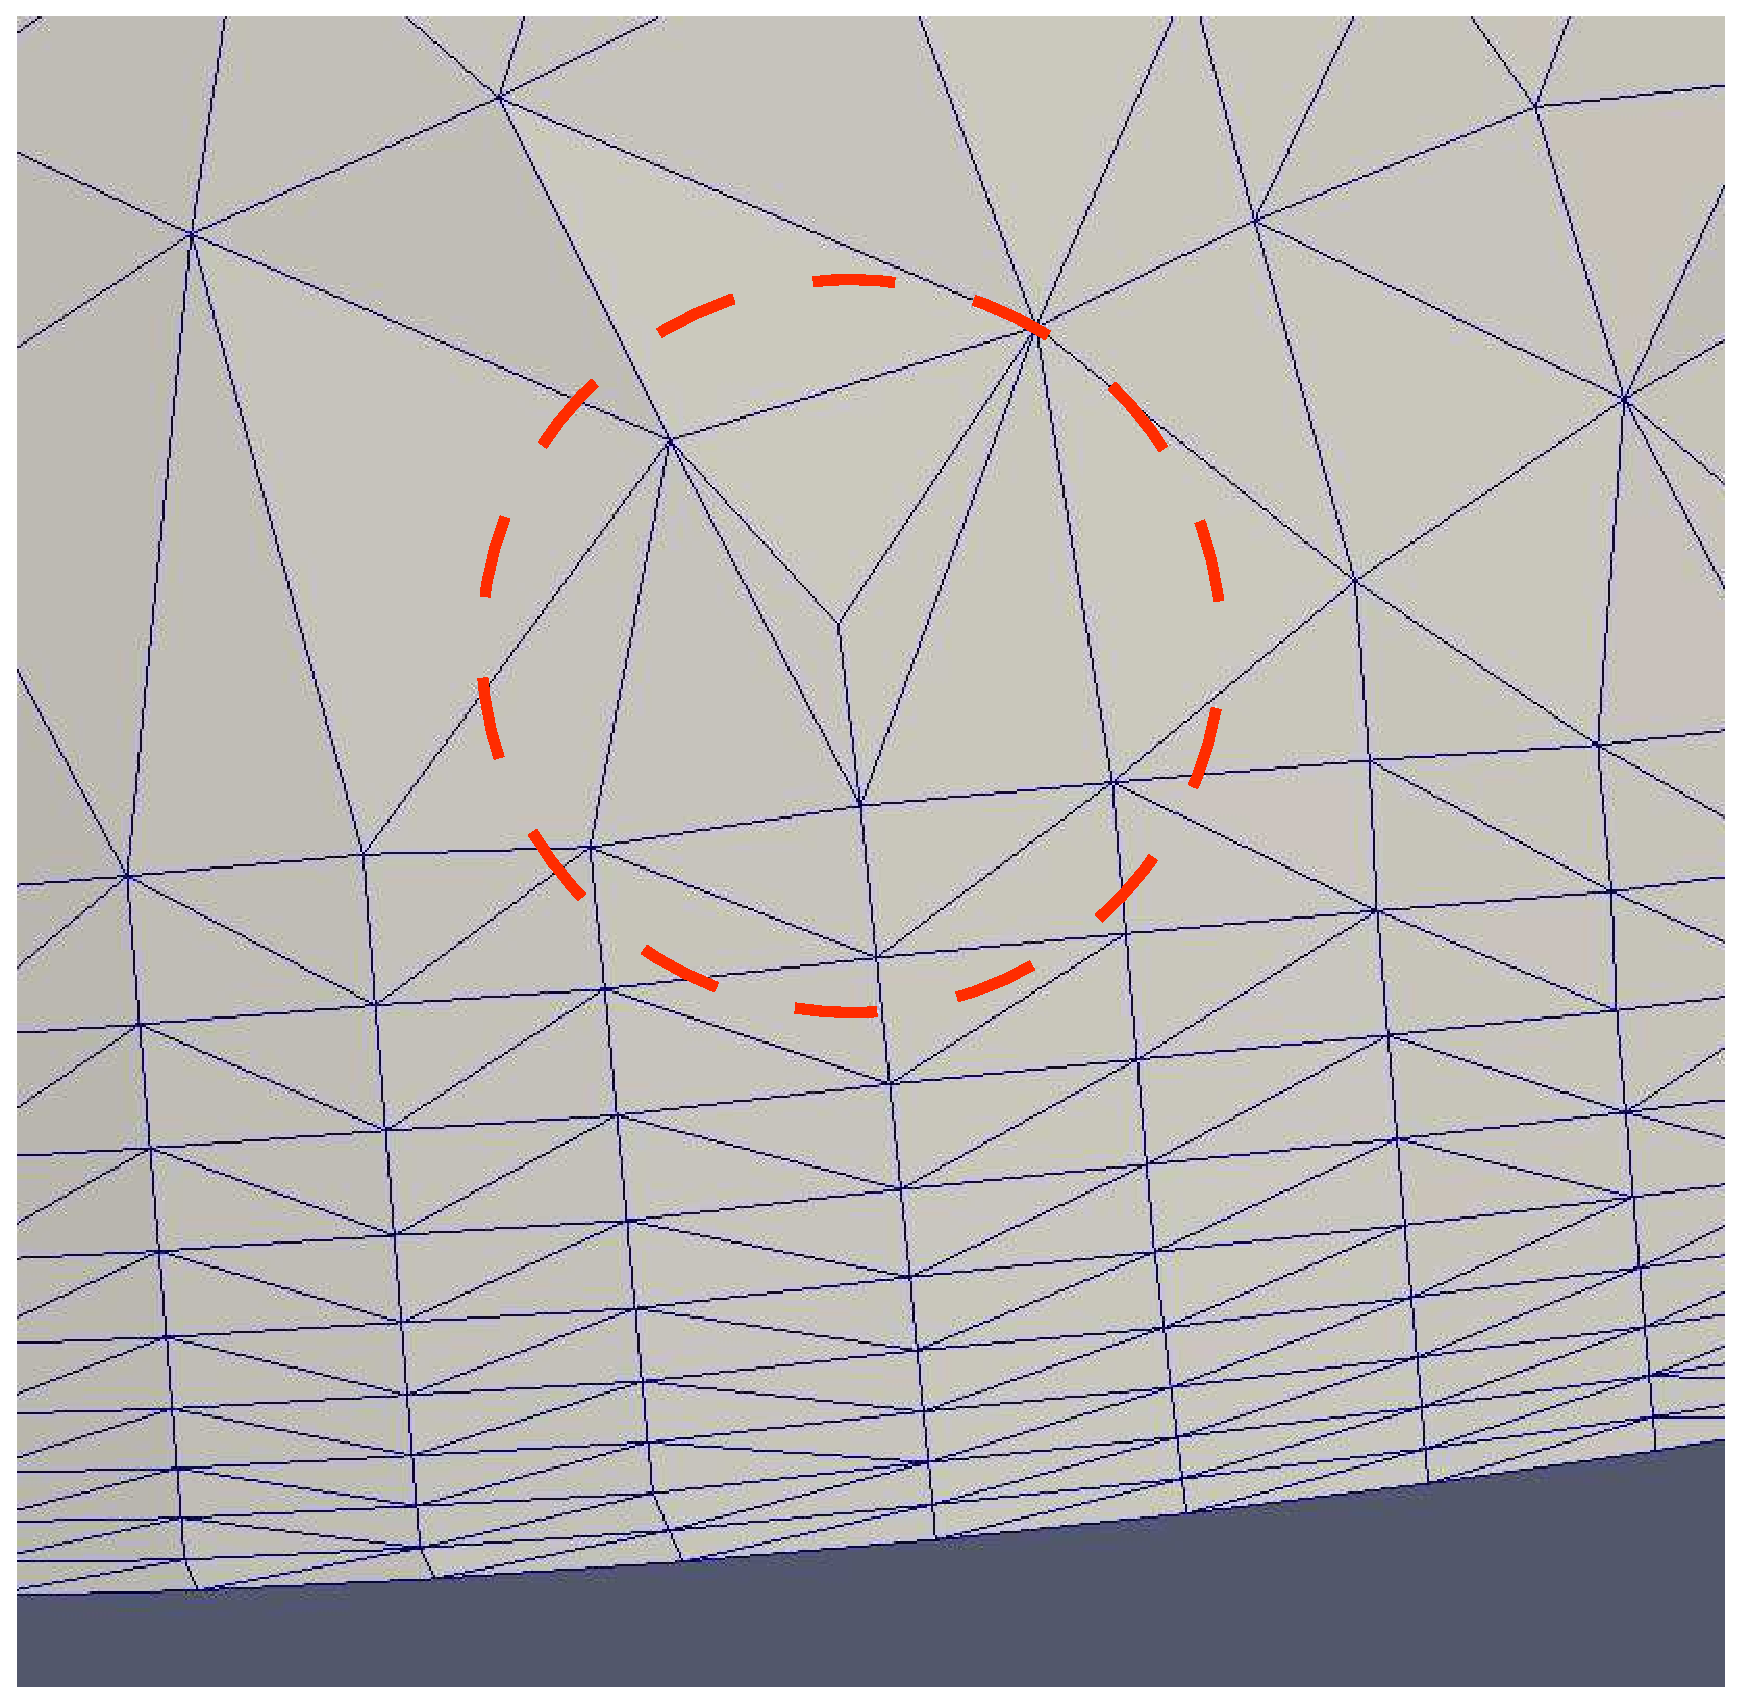
\includegraphics[width=.8\linewidth]{img/m1/point-insertion-swapping/point-inserted.eps}
  \caption{}
  \label{point-insert2}
\end{subfigure}
\begin{subfigure}{.5\textwidth}
  \centering
  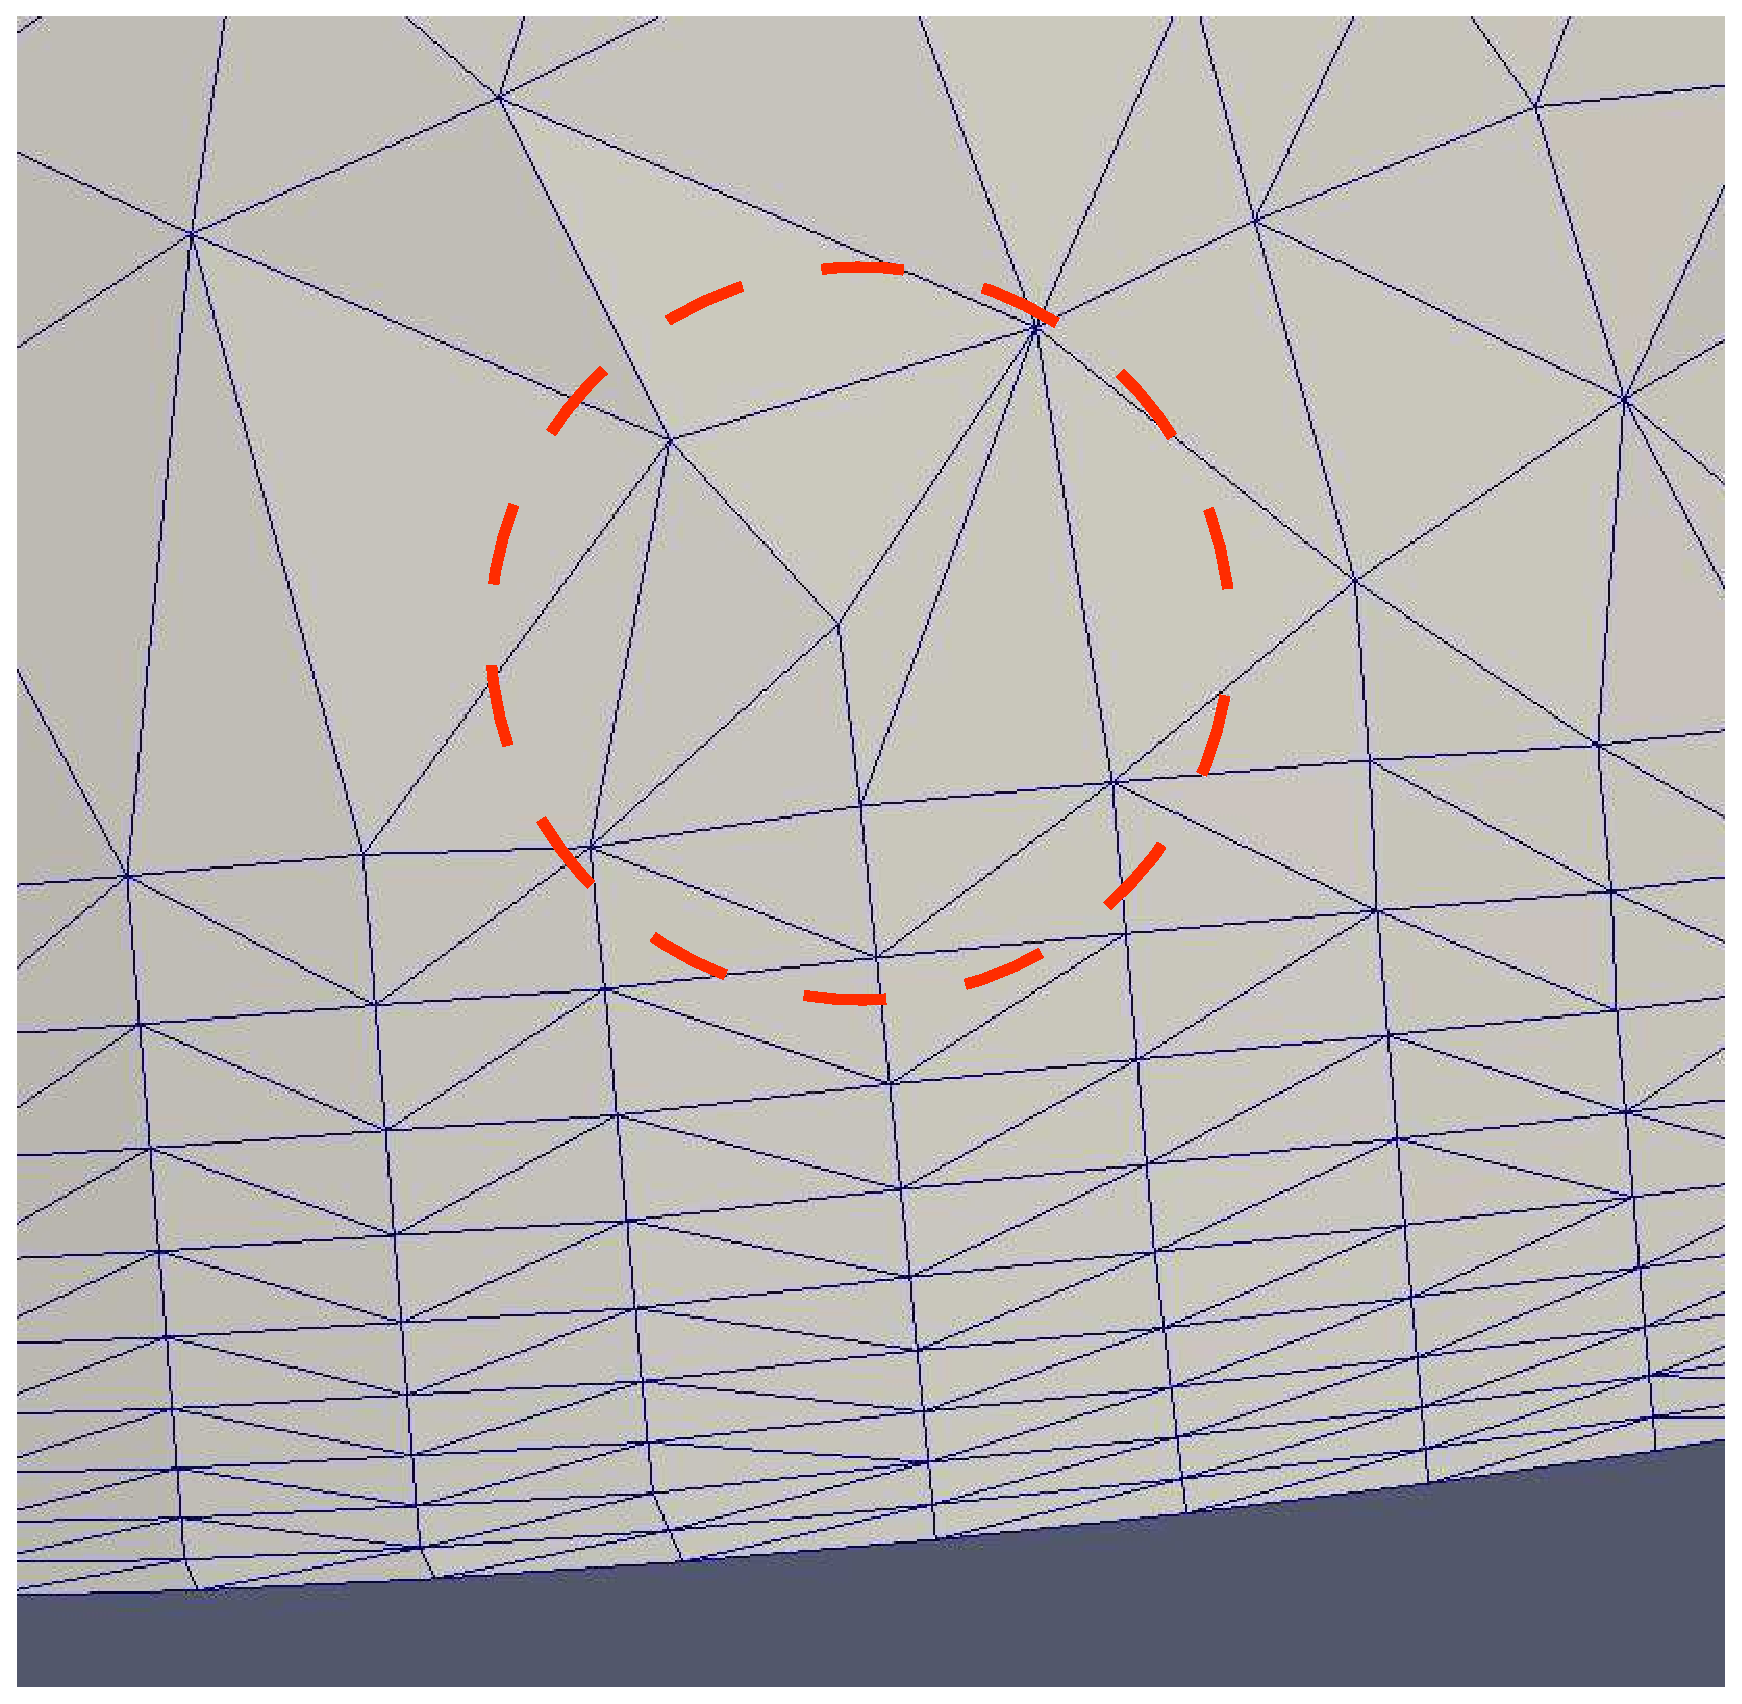
\includegraphics[width=.8\linewidth]{img/m1/point-insertion-swapping/swap1.eps}
  \caption{}
  \label{point-insert3}
\end{subfigure}%
\begin{subfigure}{.5\textwidth}
  \centering
  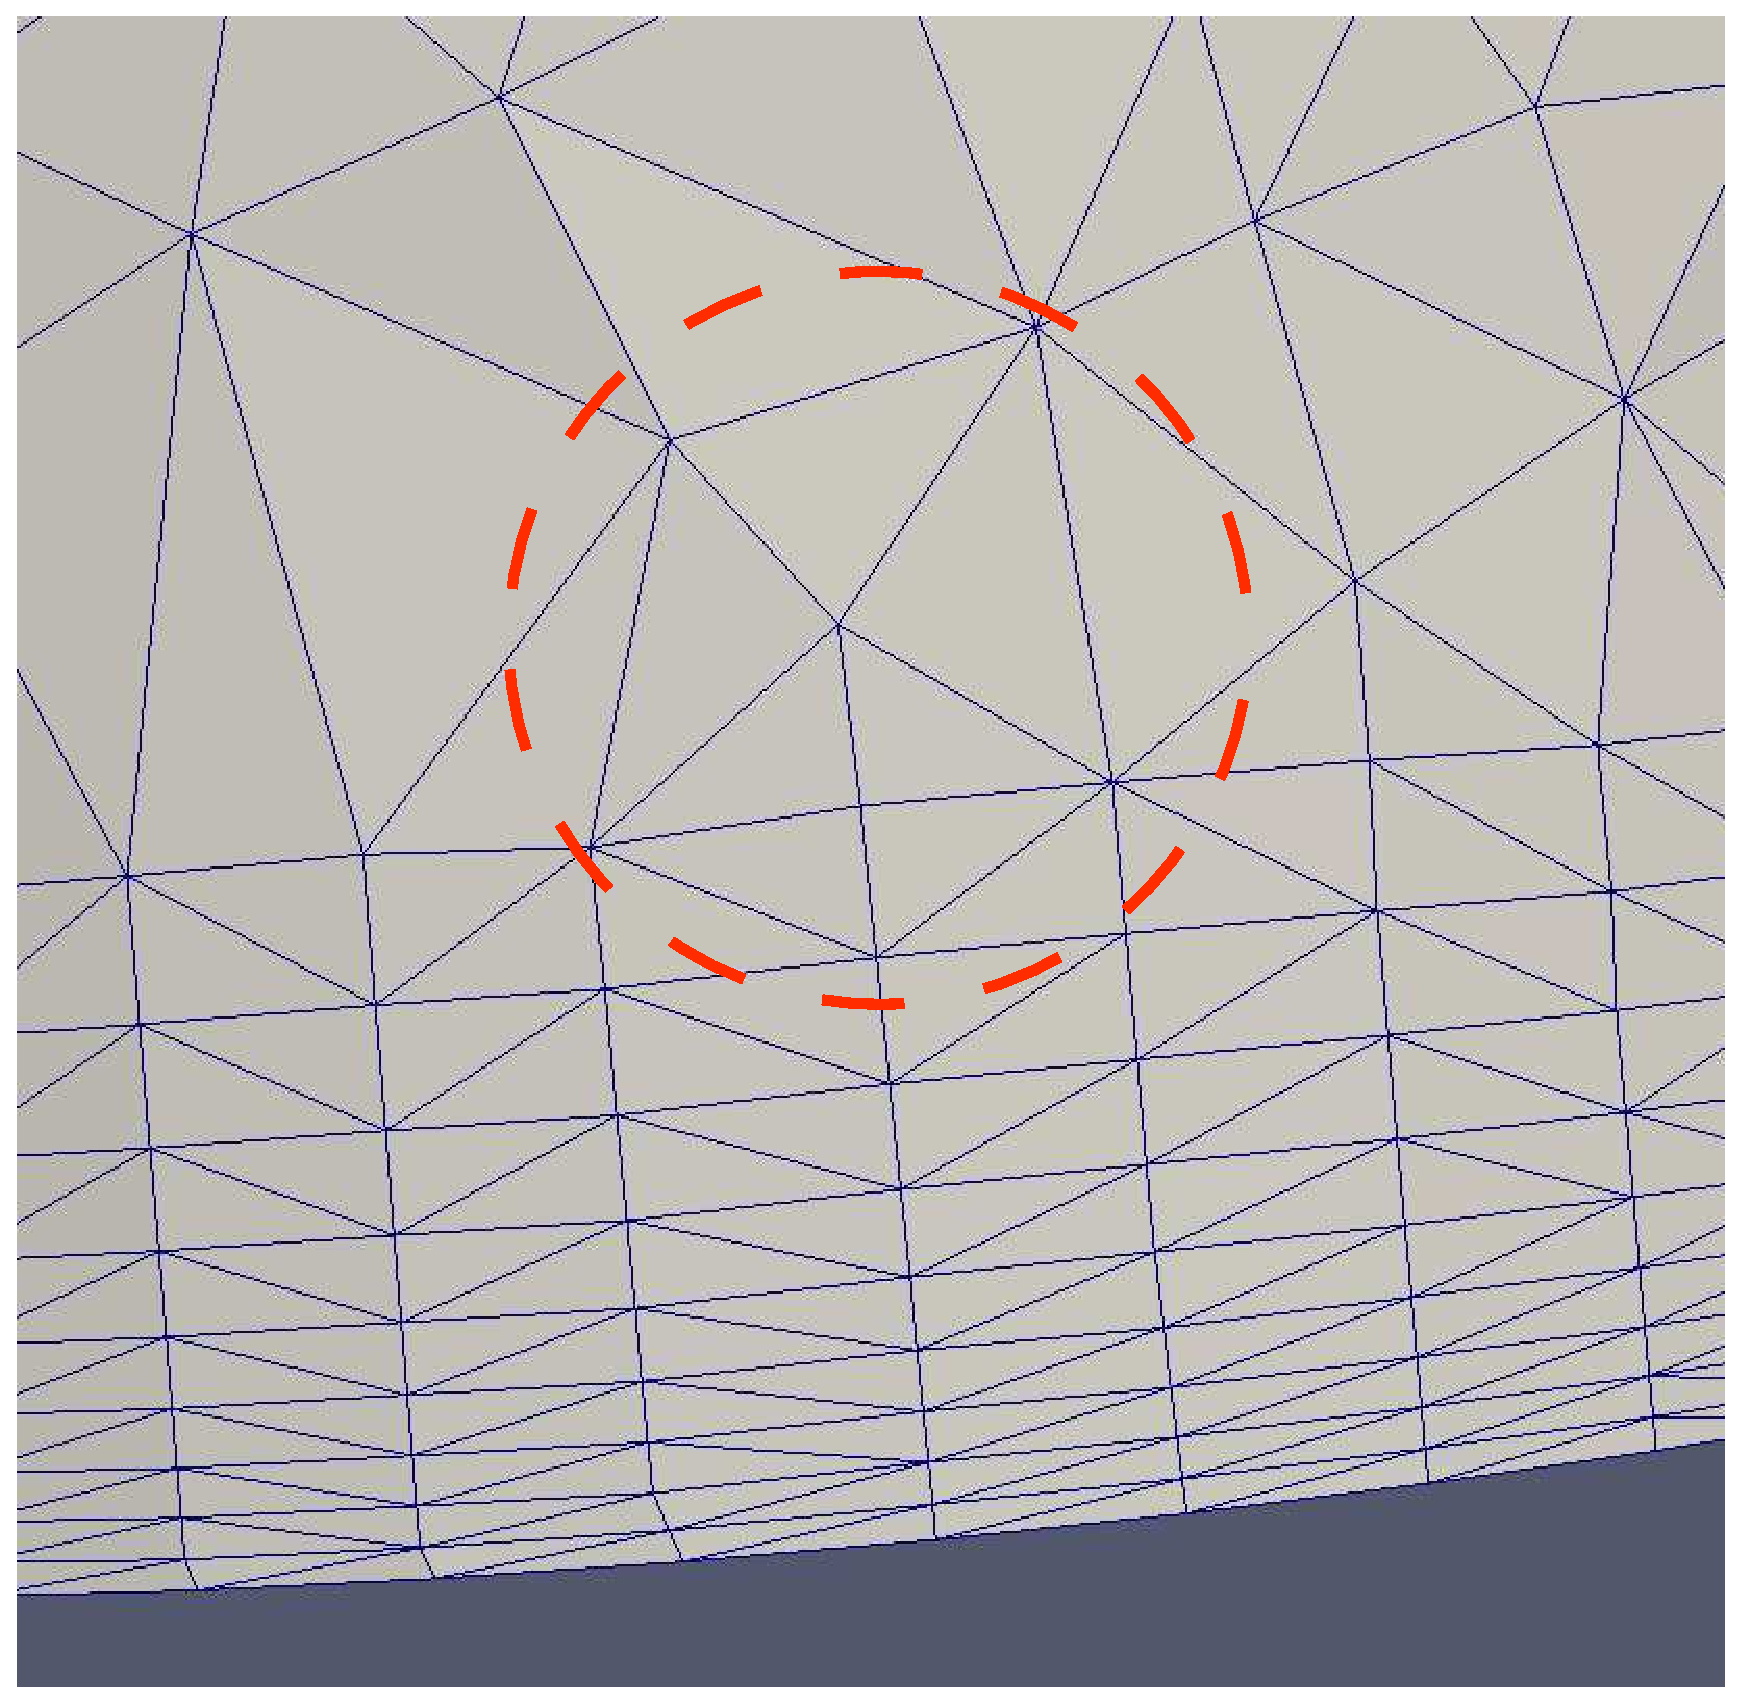
\includegraphics[width=.8\linewidth]{img/m1/point-insertion-swapping/swap2.eps}
  \caption{}
  \label{point-insert4}
\end{subfigure}
\caption{Point Insertion and local reconnection for quality shown in four steps. Red dashed circles highlight the region of the mesh that is being modified. (a) is the initial state of the mesh. A point is inserted in the mesh after extrusion from the parent point, projection onto the surface and finding the right triangle to insert. The triangle is subdivided into three new triangles as shown in (b). To improve the mesh quality after point insertion, swapping is done based on maximization of the minimum angle in a triangle. Two swaps occur as shown in figure (c) and (d) to improve mesh quality.}
\label{point-insert}
\end{figure}

A mesh observer object is initialized for the mesh data structure. The observer monitors all the changes happening to the mesh. These include the creation and deletion of vertices, edges and cells in the mesh. An edge swapping manager and quality criterion for deciding a swap are also initialized for the mesh. The primary quality criterion we chose for an edge swap is maximization of the minimum angle in the pair of triangles adjacent to the edge before and after the swap. However, only this criterion is not enough for improving surface mesh quality. This is because a better quality pair of triangles may result by edge swapping according to this criterion, however, they might deviate significantly from the underlying surface. Hence, we threshold the maximum deviation of the resultant triangles from the surface. This deviation is calculated as the angle between the normal to the triangle and the surface normal at the centriod of the triangle projected onto the surface. 

Figure \ref{deviation-surface} illustrates the deviation of a triangle $T$ formed as a result of vertex insertion from the underlying surface. Deviation of a triangle $T$ with respect to a surface $S$ is shown. $P$ is the centroid of the triangle and $P_s$ is the projection of the centroid onto the surface. $PN$ is the normal to the triangle and $P_sN_s$ is the normal to the surface at $P_s$. The interior angle $\theta$ is considered as the deviation of the triangle from the surface. An upper bound is set for $\theta$ to limit the deviation of resultant triangles from the surface.  The upper bound is set to ${30}^{\circ}$ for the surfaces meshes we are dealing with. This bound is sensitive to the refinement in the initial triangulation. A higher value of $\theta$ would be appropriate for a coarse initial triangulation while the value can be set lower for a fine initial triangulation.

We queue up the edges of the triangles affected by the insertion of the new point and do edge swapping for these edges to improve on the existing mesh. See Figure \ref{fig-pointPlacement3} and \ref{fig-pointPlacement4} for an illustration. One of the edges in the mesh is swapped to improve the quality of the triangles surrounding point Q.

%The projected point $Q$ is inserted into the advancing layer mesh. It serves as the successor or kid of point $P$ which was at the boundary curve of the sub-surface. Hence, point $Q$ would be a part of the first layer of the mesh. 

Figure \ref{point-insert} shows the process of point insertion and local reconnection in two steps in an actual mesh generation process. First, a point is inserted into the mesh at the desired location. This results in subdivision of a triangle as can be seen in figure \ref{point-insert2}. Subsequently, edge swaps occur to improve the mesh quality. Two iterations of edge swap can be seen in figure \ref{point-insert3} and \ref{point-insert4}. We do not swap the edges which comprise the front or the edge between parent and child points. Doing so would invalidate the advancing front. Hence, only interior edges of the surface or the diagonals of the quad elements generated are swapped by the face swapping algorithm. After edge swapping, the algorithm moves on to the next point in the current layer to repeat the same process.

%Before moving on to extrude other vertices in the zeroth layer, we do some edge swapping operations in the neighbourhood of the inserted vertex so as to improve the quality of the mesh in the region before we start to project other vertices from the previous layer. This process makes it easier for the vertices which remain to be extruded, to be projected inside the right triangle. Hence, it is easier to recover the next front to continue the mesh generation procedure.

\section{Front Recovery}


In an advancing layer mesh generation algorithm, an accurate representation of the boundary by anisotropic layers generated from it is very important. Also, generation of quad-elements from triangles with the right aspect ratios is far easier if we retain the boundary representation as we advance multiple layers. Hence, after all points of the parent layer are extruded, we implement a front recovery routine which recovers all edges between kid vertices.

\begin{figure}[hbt!]
\centering
\begin{subfigure}{0.5\textwidth}
  \centering
  \includegraphics[width=.9\linewidth]{img/m1/force-swapping-edge-recovery/initial-edited.eps}
  \caption{}
  \label{force-swap1}
\end{subfigure}%
\begin{subfigure}{.5\textwidth}
  \centering
  \includegraphics[width=.9\linewidth]{img/m1/force-swapping-edge-recovery/swap1-edited.eps}
  \caption{}
  \label{force-swap2}
\end{subfigure}
\begin{subfigure}{.5\textwidth}
  \centering
  \includegraphics[width=.9\linewidth]{img/m1/force-swapping-edge-recovery/swap2-edited.eps}
  \caption{}
  \label{force-swap3}
\end{subfigure}%
\begin{subfigure}{.5\textwidth}
  \centering
  \includegraphics[width=.9\linewidth]{img/m1/force-swapping-edge-recovery/swap3-edited.eps}
  \caption{}
  \label{force-swap4}
\end{subfigure}
\begin{subfigure}{.5\textwidth}
  \centering
  \includegraphics[width=.9\linewidth]{img/m1/force-swapping-edge-recovery/swap4-edited.eps}
  \caption{}
  \label{force-swap5}
\end{subfigure}
\caption{Front Recovery: Point $P_1$ and point $P_2$ here represent the two kid points generated from the boundary of the surface. We try to force a connection between the two points by iteratively swapping edges which topologically obstruct their connection. Red dashed lines represents the edge chosen to be swapped next. In (e), the green edge is the edge recovered and would serve as a part of the next front in the mesh. Note that this example is for front recovery illustration purposes and the initial boundary discretization is too coarse to get a good-quality advancing layer mesh.}
\label{force-swap}
\end{figure}

Front recovery is done by selecting a pair of points from the parent layer and then forcing an edge between the points extruded from these parent points; that is by forcing an edge between the kid vertices in the extruded layer. An edge is forced between the kid vertices by iteratively swapping any edge that lies topologically in between the two kid points. This kind of forced swapping in the mesh might seem to decrease mesh quality. However, with the right boundary discretization, it helps in giving us the high-aspect ratio elements in the mesh that we desire.

Figure \ref{force-swap} shows how exactly we recover an edge in the front by iteratively swapping the edges which obstruct the edge creation between two kid vertices, $P_1$ and $P_2$ in the figure. The edges which are topologically obstructing kid vertices $P_1$ and $P_2$ are swapped iteratively. A test is setup for each swap to avoid the flipping of triangles on the surface. After all the obstructing edges are swapped, a front edge between the kid vertices $P_1$ and $P_2$ would be recovered as shown in green in Figure \ref{force-swap5}. After forcing an edge between all the adjacent kid vertices, validity checks are run to ensure that the extruded layer is well defined and there are no discrepancies in this layer as it will serve as the parent layer for the next one. This incorporates checking the connectivity of each vertex with its adjacent edges and the connectivity of each edge with its end points. 